\documentclass[12pt, a4paper, titlepage]{article}
\usepackage[utf8]{inputenc}

% Paper settings (size, margins, etc.)
\usepackage[a4paper, total={5.8in, 8.9in}, bottom=1.4in, headsep=0.7in]{geometry}

% Text and mathematics geometry
\setlength{\parindent}{0in}
\setlength{\parskip}{12pt}
\renewcommand{\arraystretch}{1.5}

% Spacing
\usepackage{setspace}
\doublespacing

% To adjust the width of single paragraphs
\usepackage{changepage}

% Code
\usepackage{listings}
\usepackage[usenames,dvipsnames]{xcolor}

\definecolor{codegreen}{rgb}{0,0.6,0}
\definecolor{codegray}{rgb}{0.5,0.5,0.5}
\definecolor{codepurple}{rgb}{0.58,0,0.82}
\definecolor{backcolour}{rgb}{0.95,0.95,0.92}

\lstdefinestyle{mystyle}{
    backgroundcolor=\color{backcolour},   
    commentstyle=\color{codegreen},
    keywordstyle=\color{magenta},
    numberstyle=\tiny\color{codegray},
    stringstyle=\color{codepurple},
    basicstyle=\ttfamily\footnotesize,
    breakatwhitespace=true,
    breaklines=true,
    captionpos=b,
    keepspaces=true,
    numbers=left,
    numbersep=5pt,
    showspaces=false,
    showstringspaces=false,
    showtabs=false, 
    language=Python,
    frame=single,
    rulecolor=\color{codegray},
    tabsize=2,
    aboveskip=16pt,
    belowskip=24pt
}

\lstset{style=myStyle}

% Appendix
\usepackage[page, titletoc]{appendix}

% To cancel in math mode
\usepackage{cancel}

% Packages to support different mathematical features
\usepackage{amsthm}
\usepackage{amsmath}
\usepackage{amssymb}
\usepackage{mathtools}
\usepackage{amsfonts}
\theoremstyle{definition}
\usepackage{chngcntr}
\numberwithin{equation}{section}
\allowdisplaybreaks

% SVG graphics
\usepackage{svg}

% Top page titles
\usepackage{titlesec}
\titlelabel{\thetitle.\quad}

\usepackage{truncate}
\usepackage{fancyhdr}
\renewcommand{\headrulewidth}{0pt}
\renewcommand{\sectionmark}[1]{\markright{#1}}
\renewcommand{\subsectionmark}[1]{\markright{#1}}
\pagestyle{fancy}
\fancyhf{}
\fancyhead[C]{Mathematics Extended Essay: Modelling the behaviour of a pendulum}
% \lhead{\truncate{7cm}{\rightmark}}
\rfoot{\thepage}

% Language
\usepackage[british]{babel}
\hyphenation{con-si-de-ring}
\hyphenation{ma-the-ma-ti-cians}
\hyphenation{pa-ra-me-ters}

% Correct quotes display
\usepackage[style=british]{csquotes}

% Images
\usepackage{graphicx}
\graphicspath{ {./images/} }
\usepackage{wrapfig}
\usepackage{float}
\usepackage{caption}
\captionsetup{justification=centering}

% Setting up bibliography
\usepackage[
backend=biber,
sorting=nty,
citestyle=authoryear,
bibstyle=authoryear
]{biblatex}
\addbibresource{sources.bib}
\AtEveryCite{\color{MidnightBlue}}
\setlength{\bibhang}{0.4in}

\makeatletter
\newrobustcmd*{\parentexttrack}[1]{%
  \begingroup
  \blx@blxinit
  \blx@setsfcodes
  \blx@bibopenparen#1\blx@bibcloseparen
  \endgroup}
\AtEveryCite{%
  \let\parentext=\parentexttrack%
  \let\bibopenparen=\bibopenbracket%
  \let\bibcloseparen=\bibclosebracket}
\makeatother


% Setting up mathematical theorem-like entities
\newtheorem{theorem}{Theorem}
\newtheorem{corollary}{Corollary}[theorem]
\newtheorem{lemma}[theorem]{Lemma}
\theoremstyle{definition}
\newtheorem{definition}{Definition}[section]
\theoremstyle{definition}
\newtheorem{axiom}{Axiom}[section]
\newtheorem{expression}{Expression}
\newtheorem*{theorem*}{Theorem}

% Setting up the plots
\usepackage{pgfplots}
\pgfplotsset{width=0.7\textwidth,compat=1.9}

% Automatic hyper-referencing
\usepackage{hyperref}
\hypersetup{
    colorlinks=true,
    linktoc=all, 
    linkcolor=blue,
    pdftitle={How can the behaviour of a pendulum be modelled mathematically?},
    citecolor=MidnightBlue
}

% Coloring the text
\usepackage{soul}

% Coloring the math
\newcommand{\mathcolorbox}[2]{\colorbox{#1}{$\displaystyle #2$}}

% More mathematical symbols
\usepackage{commath}
\newcommand{\Lim}[1]{\raisebox{0.5ex}{\scalebox{0.8}{$\displaystyle \lim_{#1}\;$}}}

% Blackboard style
\usepackage{bbm}

% Tables
\usepackage{multirow}
\usepackage{array}
\usepackage{tabu}
\usepackage{booktabs}

% Accents
\usepackage{accents}

% Section and subsection title formats
\titleformat{\section}
{\normalfont\large\bfseries}{\thesection}{1em}{}
\titleformat{\subsection}
{\normalfont\large\bfseries}{\thesubsection}{1em}{}

% Black frame
\usepackage[contents=]{background}
\usepackage{lastpage}
\usetikzlibrary{calc}
\SetBgScale{1}
\SetBgAngle{0}
\SetBgColor{black}
\SetBgOpacity{1}

% Fancy boxes and parboxes
\usepackage{fancybox}

% No widow lines
\usepackage[all]{nowidow}

% Footnotes to bottom
\usepackage[bottom]{footmisc}

\begin{document}

\begin{titlepage}
    \centering % Centers page
    % \tikz[overlay, remember picture] \draw[thin] ([xshift=2.5cm,yshift=-2.5cm]current page.north west) rectangle ([xshift=-2.5cm,yshift=2.5cm]current page.south east);
    \tikz[overlay, remember picture] \draw[line width=1pt] ([xshift=2.35cm,yshift=-2.35cm]current page.north west) rectangle ([xshift=-2.35cm,yshift=2.35cm]current page.south east);
    
    \vspace*{180pt}
    \normalsize{{Mathematics Extended Essay\\}}
    \LARGE{How can the behaviour of a pendulum\\[0pt]be modelled mathematically?}\\
    \vspace{0.5\baselineskip}
    \small\TeX\verb+count+ word count: 3991
    \vspace*{\fill}
\end{titlepage}
\SetBgContents{
\begin{tikzpicture}[overlay,remember picture]
\draw [line width=1pt]
    ($ (current page.north west) + (0.4in,-0.9in) $)
    rectangle
    ($ (current page.south east) + (-0.4in,0.4in) $);
\end{tikzpicture}}
\pagenumbering{roman}
\doublespacing
\vspace*{\fill-0.75in}
\section*{\hfill Acknowledgements\hfill}
I cannot express enough gratitude for my teacher Jesús García de Jalón, who showed me the true beauty of mathematics. Without his teachings, I would not have been able to understand a fraction of the bibliography of this paper.

I must also thank my peer Alexander Paul Brodbelt, because without his example I would not have dared to undertake this project. His support has been and is invaluable to me.
\vspace*{\fill+0.75in}

\newpage\singlespacing
\tableofcontents\newpage
\renewcommand{\listfigurename}{List of figures}
\listoffigures\newpage
\doublespacing
\pagenumbering{arabic}
%\footnote{Although the Latin \textit{pendulum} takes \textit{pendula} as the neuter plural, English typically uses \textit{pendulums} as plural, and so will this paper.}
\section{Introduction}
Pendulums are a common object of fascination by physicists and mathematicians. The history of the study of pendulums perhaps begins with Galileo's observations on the relation between the duration of a swing, or period, and the swing amplitude, and stretches through fields such as fractal geometry or music, up to quantum mechanics. \parencite[pp. 1-6]{pendulum} Mathematically, pendulums can be reduced to models, even if the complexity of the real world results in the impossibility of perfectly describing the system through equations and functions. Even so, it is fundamental for the study of these objects to devise models that help explain how they behave.

Furthermore, the application of mathematics to real-world problems helps explore the behaviour of the world that surrounds us, and often opens up new areas of exploration within mathematics themselves. Due to this, mathematics and physics are intrinsically linked; while physics needs mathematics to describe phenomena, mathematics benefits from physics as it provides challenging problems that require the introduction of new mathematical concepts, expanding mathematics itself.

For this reason, the problem of pendulums is interesting. There is a simple solution to the problem; in fact, this is the solution that is taught in high school physics courses. Nonetheless, this basic model fails to contain the intricacies of the motion of a pendulum. Those can be approached by discarding approximations, but the problem suddenly becomes more complicated, and begs the introduction of mathematical concepts that extend beyond high school curriculums.

\subsection{Methodology}
In order to explore the concept of a pendulum, some of the knowledge from the physics course has been applied, especially regarding the forces that act on the system and the concept of simple harmonic motion. Bibliographic resources have been employed in order to understand and explain mathematical concepts such as differential equations, and apply them to the problem.

So as to put the mathematical models into practice and evaluate their behaviour with diverse parameters, I simulated them through phase portraits (see section \ref{phase_portraits}) using Python. The source code of all the simulations can be found in appendix \ref{sec:app1}.

The general approach that I will follow is:
\begin{enumerate}
\item \textbf{Understand the problem:} analyse characteristics and types of pendulums, identify the different quantities that interact within them, and focus on specific approaches.
\item \textbf{Introduce the mathematical background:} provide a sufficient understanding of differential equations, which are needed for the approaches identified previously.
\item \textbf{Develop the models:} develop the different mathematical models by applying the understanding of pendulums and the tools provided by differential equations.
\item \textbf{Analyse the models critically:} draw conclusions from the models, and identify which models are most fitting for different situations.
\end{enumerate}

\section{First approach to pendulums}
\subsection{What is a pendulum?}
\begin{figure}[H]
    \centering
    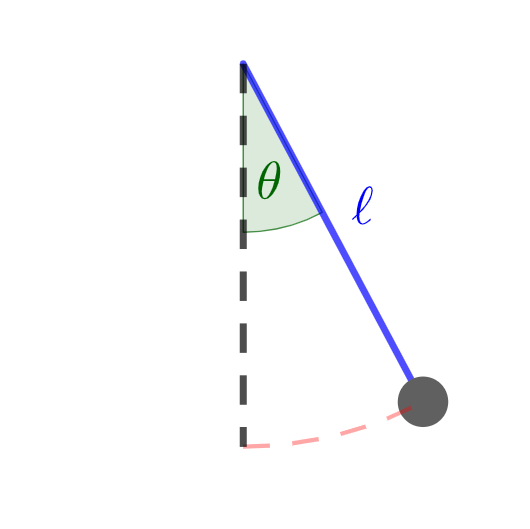
\includegraphics[scale=0.7]{pendulum2.png}
    \caption{Pendulum.}
    \label{fig:pendulum}
\end{figure}
A pendulum is a system formed by a mass that swings from a string or rod in a periodical motion. Figure \ref{fig:pendulum} shows a diagram of a pendulum, where $\theta$ is the amplitude and $\ell$ is the length of the string or rod. Pendulums can be classified according to three properties: \parencite[p. 9]{pendulum}
\begin{enumerate}
\item An \textbf{ideal} or \textbf{simple pendulum} has a mass that is concentrated in one single point of space and has a string or rod that is inelastic, i.e. does not stretch or compress. The opposite is a \textbf{real pendulum}, where the mass and elasticity of the string or rod are considered.
\item An \textbf{approximated pendulum} applies a mathematical approximation, thus simplifying the calculations; it is only valid for small angles $\theta$. The opposite is an \textbf{exact pendulum}, which does not approximate and is valid for all angles $\theta$ but does not allow for a simple analytical solution.
\item An \textbf{undamped pendulum} is one where no energy is lost, so the pendulum continues its motion permanently. The opposite is a \textbf{damped pendulum}, where energy is lost due to friction and the motion slows down as time passes.
\end{enumerate}
Real pendulums, due to their complexity, are out of the scope of this paper, but both approximated and exact pendulums, and both undamped and damped pendulums, will be considered.

\subsection{The forces acting on pendulums}
\begin{figure}[H]
    \centering
    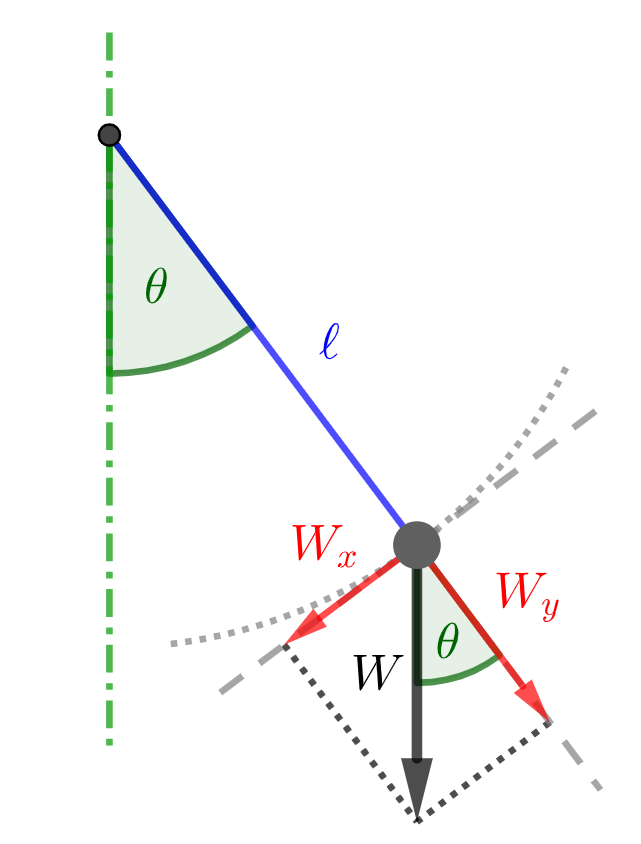
\includegraphics[scale=0.8]{force.png}
    \caption{Simple force diagram of a pendulum.}
    \label{fig:force}
\end{figure}
A way to understand the motion of a pendulum is to consider the forces that direct its movement, as shown in figure \ref{fig:force}. The simplest pendulum is one exclusively driven by a constant force of weight $\vec{W}$ that always points downwards. By considering a frame of reference based on the bob or mass of the pendulum, the vector $\vec{W}$ can be separated into its components $\vec{W_x}$ and $\vec{W_y}$. To understand how these two forces direct the motion of the pendulum, we shall apply Newton's laws of motion, shown in figure \ref{fig:newton}.

\begin{figure}
\noindent\hspace*{-6pt}\setlength\fboxsep{1cm}
\shadowbox{\parbox{\textwidth-1.9cm}{%
\textbf{Newton's laws of motion:}
\begin{enumerate}
\item \textit{Newton's First Law}: A body will remain at rest or moving with constant velocity unless acted upon
by an unbalanced force.
\item \textit{Newton's Second Law}: The acceleration of a body is proportional to the force applied and inversely
proportional to its mass. Often stated as $\vec{F}=m\vec{a}$.
\item \textit{Newton's Third Law}: If body A exerts a force on body B then body B will exert an equal and opposite force on body A.
\end{enumerate}
}%
}
\caption[Newton's laws of motion]{Newton's laws of motion. \parencite[pp. 56-67]{hamper}}
\label{fig:newton}
\end{figure}

The first law helps understand that there must be an unbalanced force acting upon the mass, because the pendulum is neither at rest nor moving at constant velocity. Since the motion of the mass is in the same direction as $\vec{W_x}$, we may assume that it is the unbalanced force of the system. The vertical component $\vec{W_y}$ must therefore be balanced by an opposite force of tension by the string or rod.

We may now drop the vector notation since the unbalanced force only acts on the horizontal axis for the chosen frame of reference; it will be positive when pointing to the right and negative when pointing to the left.

The second law implies that the unbalanced force, $W_x$, must be equal to the mass of the bob multiplied by its acceleration, $W_x=ma$. Given that the weight $W$ of a body in a gravitational field is equal to its mass multiplied by the gravitational acceleration ($W=mg$), from simple trigonometry we find that $W_x=W\sin\theta$, or $W_x=mg\sin\theta$. Combining:
\begin{align}
-ma&=mg\sin\theta\\
a&=-g\sin\theta&&\text{since $m\neq0$}\label{eq:mamgsint}
\end{align}
The negative sign represents the fact that $\theta$, and therefore $\sin\theta$, always point in the opposite direction to $a$; when the pendulum swings to the right, making $\theta$ positive, $a$ will be negative so that the pendulum slows down and eventually swings back to the left.

Equation \eqref{eq:mamgsint} provides a relationship between acceleration and angle. In order to express the acceleration in terms of $\theta$, we need to consider circular motion. In circular motion, from the definition of a radian it follows that a distance over a circular arc of length $x$ is equal to the radius of such circular arc $r$ multiplied by the angle of the arc $\theta$. In a pendulum, which follows a circular path, $r=\ell$, so:
\begin{align}
x&=\ell\theta\label{eq:slt}\\
\frac{d^2x}{dt^2}&=\ell\frac{d^2\theta}{dt^2}&&\text{differentiating twice with respect to $t$}\\
a&=\ell\ddot{\theta}&&\text{expressing derivatives as quantities}\label{eq:alt}
\end{align}
Equation \eqref{eq:alt} enables us to replace $a$ in equation \eqref{eq:mamgsint} by a quantity directly related to $\theta$, its second derivative $\ddot{\theta}$. This quantity is called angular acceleration, because it expresses the rate of change in angular velocity over time. In turn, angular velocity, $\frac{d\theta}{dt}$ or $\dot{\theta}$, expresses the rate of change in angle $\theta$ over time. Thus, substituting \eqref{eq:alt} into \eqref{eq:mamgsint}:
\begin{align}
\ell\ddot{\theta}&=-g\sin\theta\label{eq:ltgst}\\
\ddot{\theta}&+\frac{g}{\ell}\sin\theta=0&&\text{rearranging and dividing by $\ell$}\label{eq:diffeq1}
\end{align}
Equation \eqref{eq:diffeq1} leads us to an impasse. The unknown $\theta$, a function of $t$, appears as both itself and its second derivative, eliminating the possibility of isolating $\theta$ on one side of the expression. Different approaches to this obstacle will be explored in further sections.

\section{Differential equations}
Equation \eqref{eq:diffeq1} is the differential equation that describes the behaviour of a simple exact pendulum. Differential equations are a type of equation in which both a function and any of its derivatives are unknown. An example of a differential equation is one where the rate of change of a function is proportional to the function itself:
\begin{align}
y'=ry\label{eq:exp}
\end{align}
The type of differential equation that concerns pendulums is ordinary differential equations (ODEs), which contain only ordinary derivatives, in the form $y^{(n)}$ using Lagrange's notation, $\overset{n}{y}$ in dot notation (the preferred notation throughout this paper), or $\frac{d^ny}{dt^n}$ using Leibniz's.

\subsection{Ordinary differential equations}
Ordinary differential equations can be divided into linear and non-linear, a distinction which is particularly important in pendulums. Linear ODEs are typically easier to solve analytically, and are characterised by being a linear combination of a function and its derivatives: \parencite[p. 5]{ode}
\begin{align}
a_n \overset{n}{y} + a_{n-1} \overset{n-1}{y} + a_{n-2} \overset{n-2}{y} + \hdots + a_2 \dot{y} + a_1 y + a_0 = 0
\end{align}
The quantities $a_x$ may be functions of the dependent variable $t$, but not of the function $y$ itself; they may also be real numbers.

Differential equations are further identified by their highest derivative; that is, the equation $\ddot{y}+2\dot{y}=3$ is of second order because its highest derivative is $\ddot{y}$. The order of an ODE helps determine which methods to apply for resolution. \parencite[p. 4]{firstcourse}

Differential equations are often difficult to solve. In order to demonstrate how an ODE may be approached, let us find a general solution for a first order linear ODE in the form $y'=ay+b$, where $t\mapsto y$ and $a, b\in\mathbb{R}$: \parencite[pp. 7-8]{ode}
\begin{align}
y'&=a\left(y+\frac{b}{a}\right)&&\text{by factorising $a$}\\
\left(y+\frac{b}{a}\right)'&=a\left(y+\frac{b}{a}\right)&&\text{by considering that $\left(y+\frac{b}{a}\right)'=y'$}\\
a&=\frac{\left(y+\frac{b}{a}\right)'}{\left(y+\frac{b}{a}\right)}\\
a&=\frac{\bar{y}'}{\bar{y}}&&\text{by replacing $y+\frac{b}{a}$ by $\bar{y}$}\\
\int a\ dt&=\int\frac{\bar{y}'}{\bar{y}}dt&&\text{integrating on both sides}\\
at+C&=\ln\abs{\bar{y}}\\
\bar{y}&=\pm e^{at+C}\\
y+\frac{b}{a}&=\pm e^{at+C}&&\text{by replacing back $\bar{y}=y+\frac{b}{a}$}\\
y&=\pm e^Ce^{at}-\frac{b}{a}\\
y&=ce^{at}-\frac{b}{a}&&\text{where $c\in\mathbb{R}$}
\end{align}
The function $y=ce^{at}-\frac{b}{a}$, with $c$ being an arbitrary constant, is the solution of a first order linear ODE in the form $y'=ay+b$. If, for example, we apply this to equation \eqref{eq:exp}, we observe that it is a general exponential function:
\begin{align}
y'&=ry\\
a&=r,\ b=0\\
y&=ce^{rt}-\frac{0}{r}\\
y&=ce^{rt}
\end{align}
And, in fact, exponential functions are defined by the property we expressed in the differential equation: the rate of change is proportional to the function itself.

\subsection{Second order linear ODEs}
Equation \eqref{eq:diffeq1} is a second order ODE. It is not a linear combination of the function $\theta(t)$ and its derivatives, since $\theta$ appears inside another function, $\sin\theta$; therefore, it is a non-linear ODE. However, by approximating $\sin\theta$ to $\theta$, as will be demonstrated in section \ref{approx_pendulum}, equation \eqref{eq:diffeq1} can be transformed into a second order linear ODE. Thus, it will be useful to explore how they are solved.

\subsubsection{First approaches}\label{firstapproaches}
Let us start with a very simple case:
\begin{align}
\ddot{u}+u&=0&&\text{where $u$ is a function of $x$}\label{eq:simpled2}
\end{align}
It is useful to think of this problem as the question: which function, when differentiated twice, yields something which cancels out with itself? A solution could be a sine function, because the derivatives of $\sin x$ cycle between $\cos x$, $-\sin x$, $-\cos x$, back to $\sin x$, etc. Thus, substituting $u=\sin x$ into equation \eqref{eq:simpled2}:
\begin{align}
(\sin x)''+\sin x=-\sin x+\sin x=0
\end{align}
The function $\cos x$ follows the same derivative cycle, and thus is also a solution:
\begin{align}
(\cos x)''+\cos x=-\cos x+\cos x=0
\end{align}
Furthermore, any expression where the solution function is multiplied by any real arbitrary factor $c$ is also a solution:
\begin{align}
[cf(x)]''+cf(x)&=c[f(x)]''+cf(x)\\
&=c[f''(x)+f(x)]\\
&=c\cdot 0=0
\end{align}
We might observe that this is because of the property of derivatives where $\frac{d}{dx}ku=k\frac{d}{dx}u$, so the constant may always be factored out. Similarly, the property of derivatives where $\frac{d}{dx}(u+v)=\frac{d}{dx}u+\frac{d}{dx}v$ implies that for any number of solutions $y_n$, any linear combination of them will also be a solution. \parencite{mse} Let us show this for equation $y''+py'+qy=0$ with solutions $y_1$ and $y_2$:
\begin{gather}
y_1''+py_1'+qy_1=0\hspace{1cm}\text{and}\hspace{1cm}y_2''+py_2'+qy_2=0\\
(c_1y_1+c_2y_2)''+p(c_1y_1+c_2y_2)'+q(c_1y_1+c_2y_2)\\
=c_1(y_1''+py_1'+qy_1)+c_2(y_2''+py_2'+qy_2)\\
=c_1\cdot0+c_2\cdot0=0
\end{gather}
Therefore, $c_1y_1+c_2y_2$, a linear combination of solutions $y_1$ and $y_2$, is also a solution. This principle is called \textit{principle of superposition} {\parencite{superposition}}, and is useful when considering a more general case of a second order linear ODE.

\subsubsection{Generalisation}\label{generalisation}
Let us now consider a more general case:
\begin{align}
y''+py'+qy&=0\label{eq:2ngeneral}
\end{align}
We may try to approach it through exponential functions, given that their derivatives resemble them too, just like with trigonometric functions. If $y=e^{rx}$, $y'=re^{rx}$ and $y''=r^2e^{rx}$:
\begin{align}
r^2e^{rx}+pre^{rx}+qe^{rx}&=0\\
r^2+pr+q&=0&&\text{since $e^a\neq0$}\label{eq:charpoly}
\end{align}
Polynomial \eqref{eq:charpoly} is called the \textit{characteristic polynomial} of the differential equation. \parencite[pp. 102-103]{ode} If it has solutions $r_1$ and $r_2$, in terms of $p$ and $q$, then equation \eqref{eq:2ngeneral} has solutions $y_1=e^{r_1x}$ and $y_2=e^{r_2x}$. From the principle of superposition, $y=c_1e^{r_1x}+c_2e^{r_2x}$ is also a solution.

If $r_1$ and $r_2$ are complex roots in the form $a+bi$ and $a-bi$, then from the conjugate root theorem the solutions $y_1$ and $y_2$ will be:
\begin{align}
y_1&=e^{(a+bi)x}\\
y_2&=e^{(a-bi)x}
\end{align}
Using Euler's formula, $e^{ix}=\cos x+i\sin{x}$:
\begin{align}
y_1=e^{ax}e^{ibx}=e^{ax}(\cos{bx}+i\sin{bx})\\
y_2=e^{ax}e^{-ibx}=e^{ax}(\cos{bx}-i\sin{bx})
\end{align}
Since we are not looking for complex solutions, we may apply the principle of superposition with $y_1$ and $y_2$ to find real solutions. Adding $y_1$ and $y_2$ results in the following:
\begin{align}
y_1+y_2&=e^{ax}(\cos{bx}+i\sin{bx})+e^{ax}(\cos{bx}-i\sin{bx})\\
&=e^{ax}(\cos{bx}+i\sin{bx}+\cos{bx}-i\sin{bx})\\
&=2e^{ax}\cos{bx}
\end{align}
Hence, $2e^{ax}\cos{bx}$ and therefore $e^{ax}\cos{bx}$ is a solution. \parencite{paul} Replicating the process for the subtraction of $y_2$ from $y_1$ results in $2ie^{ax}\sin{bx}$ being a solution, and thus $e^{ax}\sin{bx}$ too. We may express a general real solution as:
\begin{align}
e^{ax}(c_1\cos{bx}+c_2\sin{bx})
\end{align}
\subsection{Initial values}
Constants $c_1$ and $c_2$ are related to the initial values of the solution function and its derivatives. In section \ref{firstapproaches}, we observed that second order differential equations in the form $\ddot{y}+y=0$ had solutions $y=\sin x$ and $y=\cos x$. From the principle of superposition, $y=c_1\cos x+c_2\sin x$ is a solution. If we define $y(0)=y_0$ and $\dot{y}(0)=\dot{y_0}$, we may conclude that $y_0=c_1\cos 0+c_2\sin 0=c_1$, and $\dot{y_0}=-c_1\sin 0+c_2\cos 0=c_2$. Thus, we express the solution as:
\begin{align}
y=y_0\cos x+\dot{y_0}\sin x
\end{align}
This observation is important, because it will allow us to interpret the constants $c_1$ and $c_2$ when initial values are determined.
\subsection{Phase portraits}\label{phase_portraits}
A phase portrait of a system is a representation of all its possible states and developments. It is a useful tool to understand the behaviour of a system that is described through a differential equation, especially when there exists no analytical solution for it. Phase portraits depict trajectories of a system, that is, directions in which it will evolve given a specific state. They are a sort of simulation of what would happen in every possible initial state as time increases.

Phase portraits will be used throughout this paper to help extract conclusions from the different models. They will be shown as vector fields, sometimes with solution curves plotted to better understand the behaviour of the motion.

\section{An approximated pendulum}\label{approx_pendulum}
As discussed above, one possible way to approach the problem is to approximate $\sin\theta$ as $\theta$. This is helpful because it allows us to consider the motion as simple harmonic motion, and to solve equation \eqref{eq:diffeq1} analytically by \textbf{making the differential equation linear}.

\subsection{Simple harmonic motion}
Simple harmonic motion is a periodic motion where a body oscillates around an equilibrium position. SHM is characterised by the fact that the acceleration towards the equilibrium position is proportional to and of opposite sign as its displacement from the equilibrium position.
\begin{align}
a\propto-x\label{eq:apx}
\end{align}
The negative sign means that when the body moves away from the equilibrium position, the acceleration will point to the opposite direction, towards the equilibrium position. \parencite[p. 151]{hamper} Applying the approximation to a pendulum proves a close resemblance to SHM in small angles. Using the approximation, $\sin\theta\approx\theta$, on equation \eqref{eq:diffeq1}:
\begin{align}
\ddot{\theta}&=-\frac{g}{\ell}\theta\\
\frac{a}{\bcancel{\ell}}&=-\frac{g}{\ell} \frac{x}{\bcancel{\ell}}\\
a&=-\frac{g}{\ell}x\quad\implies\quad a\propto-x\label{eq:aglx}
\end{align}
\subsection{The small angle approximation}\label{sub:small}
The small angle approximation is a mathematical approximation of trigonometric functions. Figure \ref{fig:squeeze} helps gain an understanding of it:
\begin{figure}[H]
    \centering
    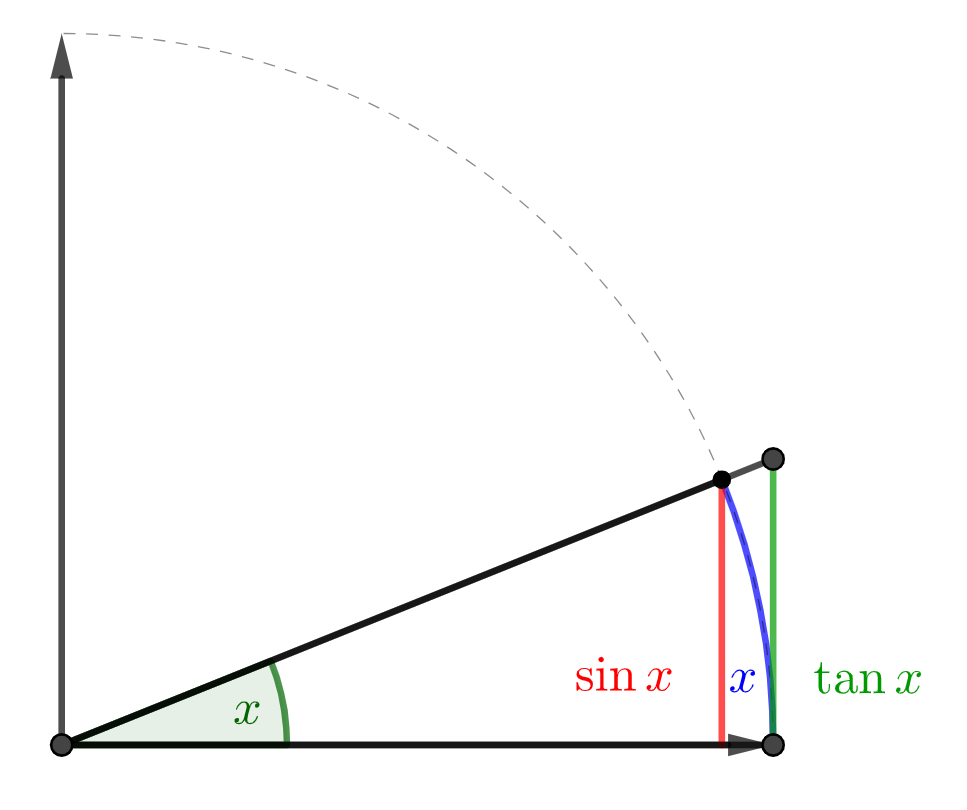
\includegraphics[scale=5]{squeeze-theorem.png}
    \caption{Squeeze theorem with trigonometric functions.}
    \label{fig:squeeze}
\end{figure}
%\newpage
\begin{theorem*}
\textit{Small angle approximation.}
\begin{adjustwidth}{2cm}{}
From figure \ref{fig:squeeze} we may deduce that, for small values of the angle $x$, $\sin{x}\leq x \leq \tan{x}$. Dividing  by $\sin{x}$ on all three functions, $1\leq \frac{x}{\sin{x}} \leq \cos{x}$.
\end{adjustwidth}
\begin{gather}
\text{If }1\leq \frac{x}{\sin{x}}\leq \cos{x}\text{ in an interval containing }x=0\text{,}\\
\text{and if }\lim_{x\to 0}{1}=1=\lim_{x\to 0}{\cos{x}},\\
\text{ then }\lim_{x\to 0}{\frac{x}{\sin{x}}}=1\label{eq:sm3}
\end{gather}
\begin{adjustwidth}{2cm}{}
Rearranging statement \eqref{eq:sm3}, \textbf{for \boldmath$x\to 0$, $\sin{x}\approx x$}.
\end{adjustwidth}
\end{theorem*}
\noindent This approximation is relatively accurate for small angles; to show this, let us calculate $\sin{\theta}$ for $\theta = \frac{\pi}{12}$ with three significant figures:
\begin{alignat*}{2}
\sin{\theta} &= \sin{\frac{\pi}{12}} &= 0.259 \\
\theta &= \frac{\pi}{12} &= 0.262
\end{alignat*}
The difference, which in this example is of slightly over $1\%$, is small enough to be neglected with small angles.

\subsection{A differential approach to SHM}
We may proceed to solve our approximated differential equation through the general method derived in section \ref{generalisation}:
\begin{align}
&\text{Differential equation:}&&\ddot{\theta}+\frac{g}{\ell}\theta=0\\
&\text{Characteristic polynomial:}&&r^2+\frac{g}{\ell}=0\\
&\text{Roots of the polynomial:}&&r=\pm\sqrt{\frac{g}{\ell}}i\\
&\text{Constants $a$ and $b$ for $r=a\pm bi$:}&&a=0,\ b=\sqrt{\frac{g}{\ell}}\\
&\text{Substitution in the formula:}&&\hspace{-24pt}\theta(t)=e^{0t}(c_1\cos{\sqrt{\frac{g}{\ell}}t}+c_2\sin{\sqrt{\frac{g}{\ell}}t})\\
&\text{Simplification and constants:}&&\hspace{-24pt}\theta(t)=\theta_0\cos{\sqrt{\frac{g}{\ell}}t}+\dot{\theta_0}\sin{\sqrt{\frac{g}{\ell}}t}\label{eq:shmmodel2}
\end{align}

Equation \eqref{eq:shmmodel2} provides a simple harmonic model for an \textbf{undamped approximated pendulum}. Figure \ref{fig:shm1} shows the graph of the function with no initial velocity $\dot{\theta_0}$, where maxima represent the maximum swing to the right, and minima do so to the left. As is to be expected, the gradient of the curve, that is, the angular velocity, has maximum magnitude when the angle is zero, which means that the bob stops moving down and starts moving up.
\begin{figure}[H]
    \centering
    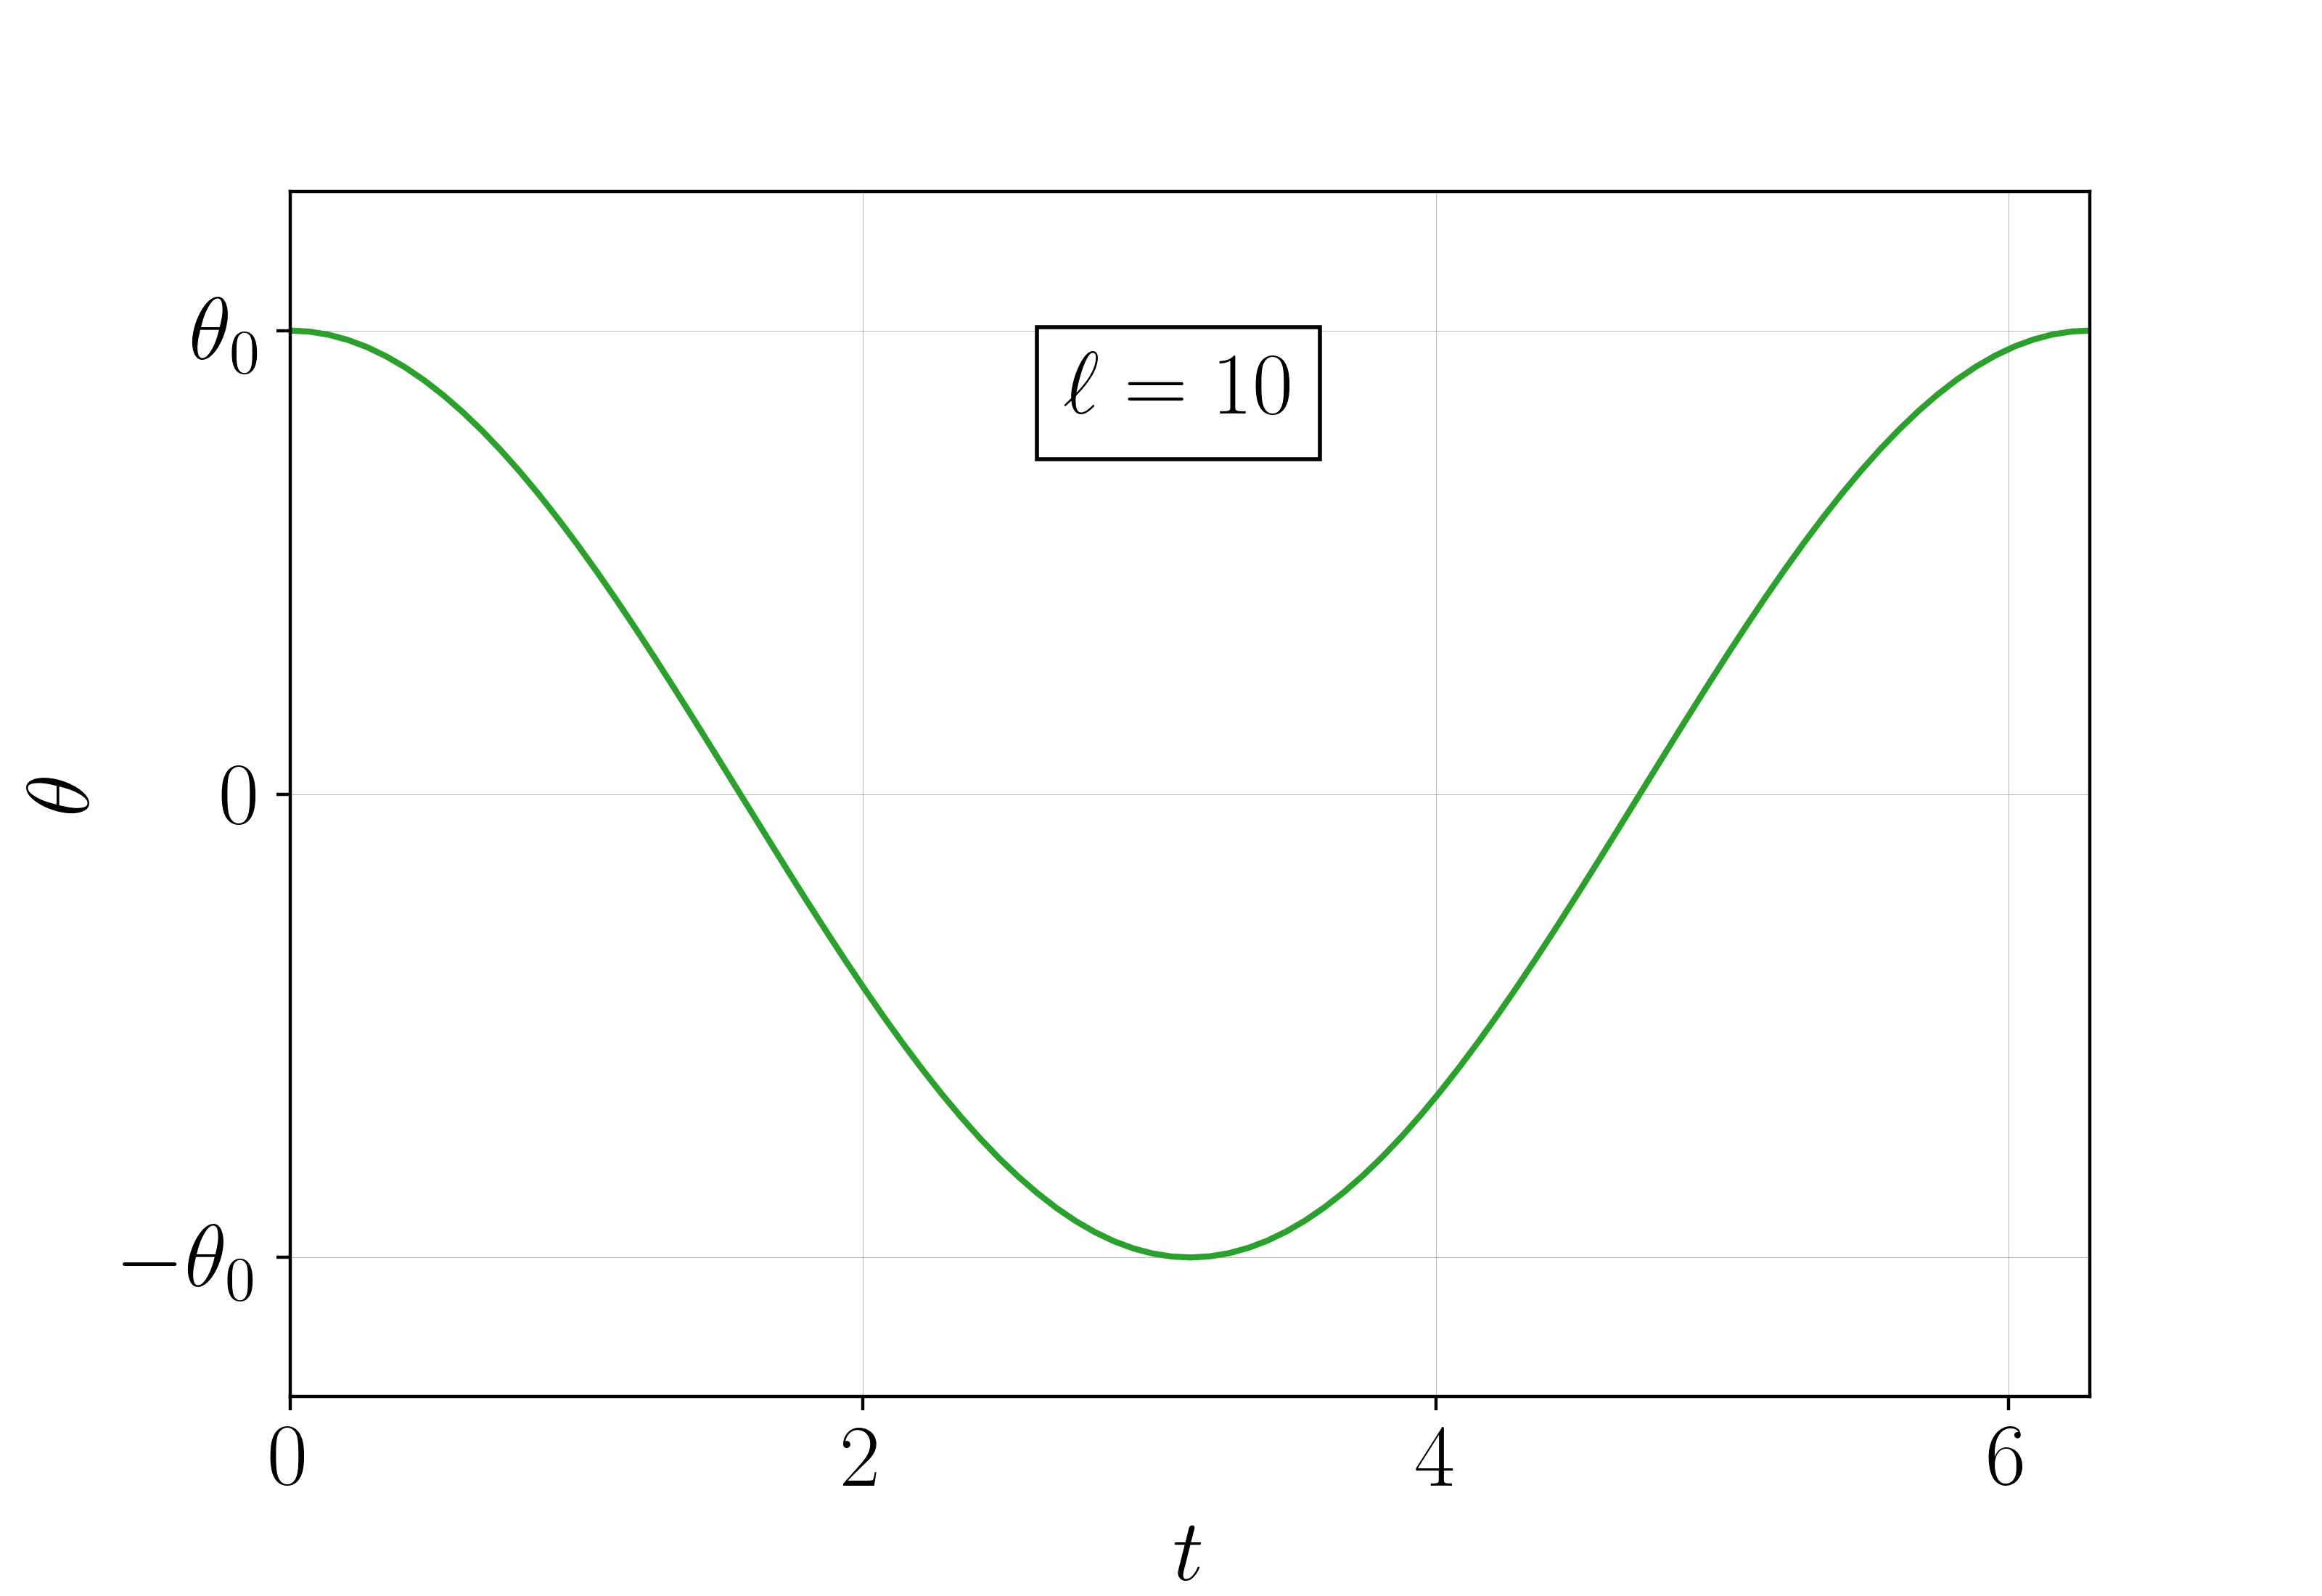
\includegraphics[scale=0.6]{shm1.png}
    \caption{Graph of $\theta(t)$ in simple harmonic motion.}
    \label{fig:shm1}
\end{figure}

We may create a phase portrait of the differential equation, with the two parameters, angle and angular velocity, as axes. They may be shown through a vector field, where the magnitude of the vector at a particular point will express the instantaneous rate of change of both quantities, that is, how they will change.

In order to create the phase portrait, with axes to represent $\theta_0$ and $\dot{\theta_0}$, it is necessary to perform a change of variable to obtain separate expression for the derivative of each of the variables. Thus, $\theta=\theta_1$ and $\dot{\theta}=\dot{\theta_1}=\theta_2$:
\begin{align}
&\ddot{\theta}+\frac{g}{\ell}\theta=0&&\text{differential equation}\\
&\dot{\theta_2}+\frac{g}{\ell}\theta_1=0&&\text{change of variables}\\[16pt]
&\hspace{-12pt}\begin{cases}
\dot{\theta_1}=\theta_2\\
\dot{\theta_2}=-\frac{g}{\ell}\theta_1
\end{cases}&&\text{system of equations}\label{eq:syseq1}
\end{align}
From that, given a point $(\theta_1, \theta_2)$, its derivative as a vector will be $\begin{bsmallmatrix}\theta_2\\[6pt]-\frac{g}{\ell}\theta_1\end{bsmallmatrix}$. Figure \ref{fig:phase_approx_simple} shows the phase portrait.
\begin{figure}[H]
    \centering
    \includesvg[scale=1]{phase_approx_simple.svg}
    \caption[Phase portrait of an undamped approximated pendulum.]{Phase portrait of a simple approximated pendulum.}
    \label{fig:phase_approx_simple}
\end{figure}
Some conclusions can be extracted from this phase portrait:
\begin{enumerate}
\item The pendulum \textbf{does not lose energy}, because after a complete swing it returns back to the original point.
\item The \textbf{angular velocity has maximum magnitude} when the \textbf{angle is zero}, which means that the pendulum moves the fastest when at its lowest point.
\item The \textbf{angle has maximum magnitude} when the \textbf{angular velocity is zero}, so the velocity vector changes its direction and therefore its sign when the pendulum reaches its highest point on either side of the motion.
\end{enumerate}


\subsection{A damped approximated pendulum}
Recalling the force diagram in figure \ref{fig:force}, the unbalanced force of an undamped pendulum is the horizontal component of weight. We may now introduce a force of friction proportional to the velocity of the pendulum: \parencite[pp. 3-4]{damped}
\begin{align}
F_{fric}=-bv
\end{align}
Where $b$ is a friction coefficient, and $v$ is the linear velocity of the pendulum. Note that the negative sign indicates that the force always acts opposite to the velocity, because it slows down the motion. We may replace the linear velocity by the angular velocity:
\begin{align}
x&=\ell\theta\\
\frac{dx}{dt}&=\ell\frac{d\theta}{dt}&&\text{differentiating with respect to $t$}\\
v&=\ell\dot{\theta}\\
F_{fric}&=-b\ell\dot{\theta}
\end{align}
\begin{figure}[H]
    \centering
    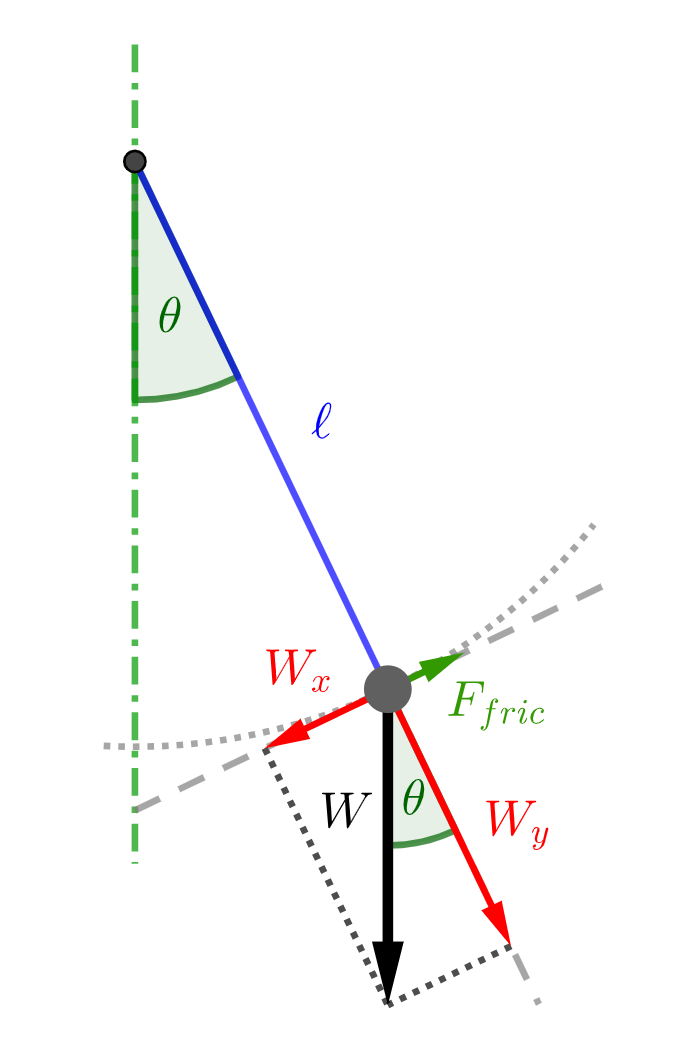
\includegraphics[scale=0.8]{force2.png}
    \caption{Force diagram of a damped pendulum.}
    \label{fig:force2}
\end{figure}
By reintroducing the force diagram adding the new force, figure \ref{fig:force2}, the total unbalanced force is the sum of all the forces that act on the body, namely the horizontal component of the weight, $W_x$, and the friction, $F_{fric}$:
\begin{align}
F_{total}&=ma=W_x+F_{fric}\\
ma&=-mg\sin\theta-b\ell\dot{\theta}\\
m\ell\ddot{\theta}&=-mg\sin\theta-b\ell\dot{\theta}&&\text{from \eqref{eq:alt}}\\
\ddot{\theta}&+\frac{b}{m}\dot{\theta}+\frac{g}{\ell}\sin\theta=0\\
\ddot{\theta}&+\frac{b}{m}\dot{\theta}+\frac{g}{\ell}\theta=0&&\text{approximating}
\end{align}
Using the characteristic polynomial, $r^2+\frac{b}{m}r+\frac{g}{\ell}=0$, and finding its roots, $r=-\frac{b}{2m}\pm\frac{1}{2}{\sqrt{\left(\frac{b}{m}\right)^2-4\frac{g}{\ell}}}$, the solution to the differential equation will be:
\begin{align}
\theta\left(t\right)=e^{-\frac{b}{2m}t}\left(c_1\cos{t\frac{1}{2}{\sqrt{\left(\frac{b}{m}\right)^2-4\frac{g}{\ell}}}}+c_2\sin{t\frac{1}{2}{\sqrt{\left(\frac{b}{m}\right)^2-4\frac{g}{\ell}}}}\right)
\end{align}
Once again, given initial values $\theta(0)=\theta_0$ and $\dot{\theta}(0)=\dot{\theta_0}$, we interpret the constants as $c_1=\theta_0$ and $c_2=\dot{\theta_0}$. Figure \ref{fig:damped1} shows a possible graph of the solution function, with the same interpretation for the maxima and the minima as in figure \ref{fig:shm1}.
\begin{figure}[H]
    \centering
    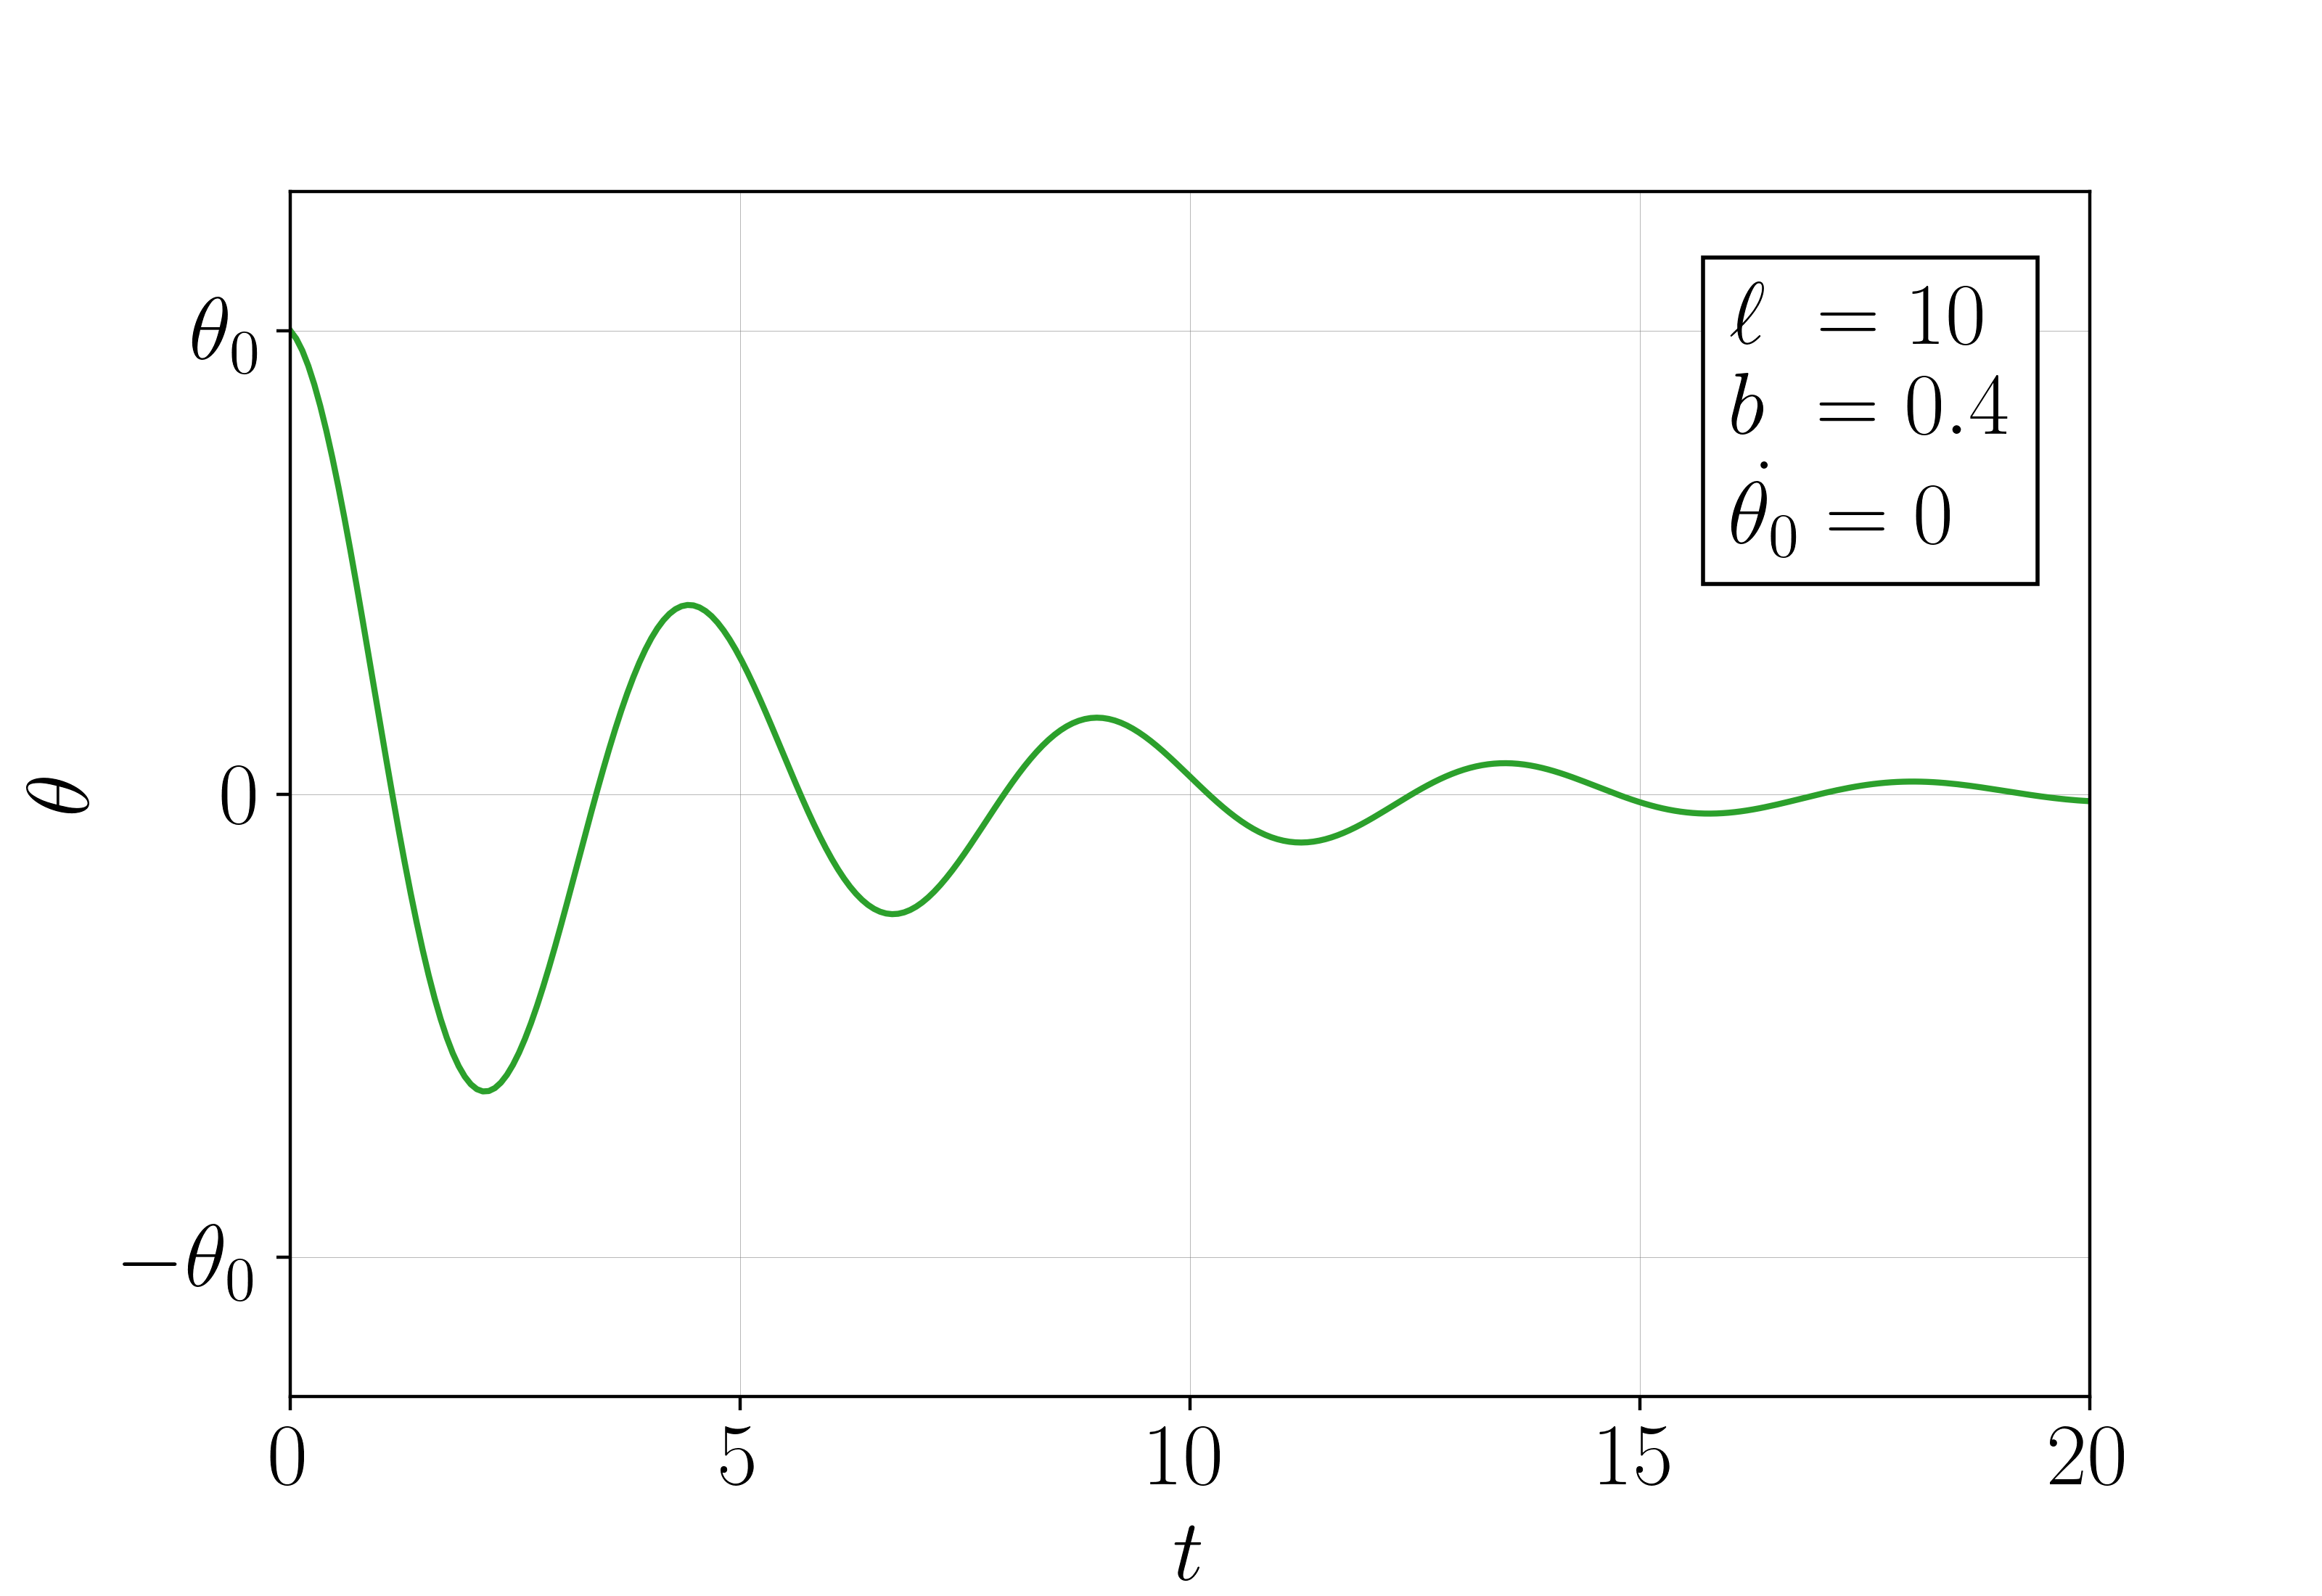
\includegraphics[scale=0.7]{damped1.png}
    \caption{Graph of $\theta(t)$ in damped motion.}
    \label{fig:damped1}
\end{figure}
There is one clear flaw with this model: even though we are accounting for some energy loss, there is an asymptote for $\theta=0$, which means that while the curve crosses zero infinite times, and gets closer and closer to zero, it never stops at it. Thus, this model is of a pendulum that loses energy but never all of it, so it never stops.

Another way of representing this model is again through a phase portrait, where given initial values for $\theta_0$ and $\dot{\theta_0}$, the rate of change, that is, the expected direction of the curve as time increases, is shown through a vector field. Through the method in \eqref{eq:syseq1}:
\begin{align}
\begin{cases}
\dot{\theta_1}=\theta_2\\
\dot{\theta_2}=-\frac{g}{\ell}\theta_1-\frac{b}{m}\theta_2
\end{cases}
\end{align}
\begin{figure}[H]
    \centering
    \includesvg[scale=1]{phase_approx_damped.svg}
    \caption{Phase portrait of a damped approximated pendulum.}
    \label{fig:phase_approx_damped}
\end{figure}
Figure \ref{fig:phase_approx_damped} shows the phase portrait with one solution curve. The solution curve spirals towards zero as it loses energy exponentially (due to the first factor of the function, $e^{at}$), but never reaches that point.

\section{An exact pendulum}
Bringing back our initial differential equations for undamped and damped pendulums:
\begin{align}
&\text{Undamped:}&&\ddot{\theta}+\frac{g}{\ell}\sin\theta=0\label{eq:undamped_exact}\\
&\text{Damped:}&&\ddot{\theta}+\frac{b}{m}\dot{\theta}+\frac{g}{\ell}\sin\theta=0\label{eq:damped_exact}
\end{align}
Since these equations are not linear, we have no tools to solve them analytically. Nonetheless, as shown previously, phase portraits contain as much information as plotted functions, and we can draw conclusions from them. Therefore, the exact pendulum will be approached through phase portrait simulations, and solution curves plotted on them.

\subsection{An undamped exact pendulum}
We can once again separate the differential equation for the undamped exact pendulum, \eqref{eq:undamped_exact}, into a system of equations through a change of variables, which will help us create its phase portrait. Replicating the process in equation \eqref{eq:syseq1}:
\begin{align}
\begin{cases}
\dot{\theta_1}=\theta_2\\
\dot{\theta_2}=-\frac{g}{\ell}\sin\theta_1
\end{cases}
\end{align}
Plotting the phase portrait  as a vector field, where a vector at point $(\theta_1, \theta_2)$ is defined by $\begin{bsmallmatrix}\theta_2\\[6pt]-\frac{g}{\ell}\sin\theta_1\end{bsmallmatrix}$, results in figure \ref{fig:phase_exact_damped_noplot}.
\begin{figure}[H]
    \centering
    \includesvg[scale=0.75]{phase_exact_simple_noplot.svg}
    \caption{Phase portrait of an undamped exact pendulum.}
    \label{fig:phase_exact_simple_noplot}
\end{figure}
This phase portrait displays more complexity than the approximated ones. Some remarkable features include:
\begin{enumerate}
\item It is \textbf{periodic}. Every $2\pi$ radians along the horizontal axis, the vector field will be the exact same.
\item It works for \textbf{any angle}, which is especially noticeable for $\theta>\pi$ or $\theta<-\pi$, where the approximated pendulum predicted a strong trend towards the origin, whereas a real pendulum will move towards the nearest stable point.
\item There are more points where the \textbf{vector magnitude is zero} than solely the origin. This hints at different points of equilibrium, or no motion:
\begin{enumerate}
\item The \textbf{unstable equilibrium points} correspond to multiples of $\pi$ (in \textcolor{red}{\textbf{red}}), where the pendulum is at the top, and are therefore unstable, because any external disturbance brings the pendulum into circling about forever.
\item The \textbf{stable equilibrium points} correspond to multiples of $2\pi$ (in \textcolor{blue}{\textbf{blue}}), where the pendulum is at the bottom, and are therefore stable, because any external disturbance sets the pendulum to oscillate slightly about the stable point.
\end{enumerate}
\end{enumerate}
\begin{figure}[H]
    \centering
    \includesvg[scale=0.75]{phase_exact_simple_plot.svg}
    \caption{Phase portrait of an undamped exact pendulum\\with various solutions plotted.}
    \label{fig:phase_exact_simple_plot}
\end{figure}
Some solution curves with different initial conditions are shown in figure \ref{fig:phase_exact_simple_plot}:\begin{itemize}
\item \textcolor{MidnightBlue}{\textbf{Curve A}} behaves similarly to an undamped approximated pendulum, because it has a low initial angular velocity, so its maximum angle is small.
\item \textcolor{Red}{\textbf{Curve B}} does not have enough initial velocity to circle around, and while it approaches the top on every swing, it never reaches it and falls back towards its initial point.
\item \textcolor{Green}{\textbf{Curve C}} gets very close to stopping (graphically, approaching the horizontal axis) every time it passes through the top, but it manages to \enquote{overcome} it and circles around forever.
\item \textcolor{Orchid}{\textbf{Curve D}} behaves like curve C, except it has higher initial angular velocity, and so it circles around forever, only slightly slowing down when it is at the top of its motion.
\end{itemize}

\subsection{A damped exact pendulum}
Once again, parallel to the method in \eqref{eq:syseq1}, we plot the phase portrait (figure \ref{fig:phase_exact_damped_noplot}) from the following system of equations:
\begin{align}
\begin{cases}
\dot{\theta_1}=\theta_2\\
\dot{\theta_2}=-\frac{g}{\ell}\sin\theta_1-\frac{b}{m}\theta_2
\end{cases}
\end{align}
The vector field will follow that a vector at point $(\theta_1, \theta_2)$ is defined by $\begin{bsmallmatrix}\theta_2\\[6pt]-\frac{g}{\ell}\sin\theta_1-\frac{b}{m}\theta_2\end{bsmallmatrix}$, resulting in figure \ref{fig:phase_exact_damped_noplot}.
\begin{figure}[H]
    \centering
    \includesvg[scale=0.75]{phase_exact_damped_noplot.svg}
    \caption{Phase portrait of a damped exact pendulum.}
    \label{fig:phase_exact_damped_noplot}
\end{figure}
Performing a similar analysis to the previous section:
\begin{enumerate}
\item It is again \textbf{periodic}.
\item There is a trend towards \textcolor{blue}{\textbf{stable equilibrium points}}, and away from \textcolor{red}{\textbf{unstable equilibrium points}}.
\item The stable equilibrium points can now be called \textbf{attractors} and the unstable equilibrium points \textbf{repellors}: \parencite{wolfram}
\begin{enumerate}
\item \textbf{Attractors} are points towards which neighbouring states approach as the system evolves.
\item \textbf{Repellors} are points from which neighbouring states move away as the system evolves.
\end{enumerate}
\end{enumerate}
\begin{figure}[H]
    \centering
    \includesvg[scale=0.75]{phase_exact_damped_plot.svg}
    \caption{Phase portrait of a damped exact pendulum\\with various solutions plotted.}
    \label{fig:phase_exact_damped_plot}
\end{figure}
Plotting again some solution curves results in figure \ref{fig:phase_exact_damped_plot}:
\begin{itemize}
\item \textcolor{MidnightBlue}{\textbf{Curve A}} starts with certain initial velocity, and oscillates from right to left in increasingly small swings without ever circling around completely.
\item \textcolor{Green}{\textbf{Curve B}} has enough initial velocity to circle around once, but gets trapped in the next cycle and so after the first full circle it starts to behave like curve A.
\item \textcolor{Orchid}{\textbf{Curve C}} starts with a somewhat high initial angle and no velocity, and it oscillates with a decreasing swing angle.
\end{itemize}
The main conclusion drawn from approximated undamped pendulums, that referred to the asymptote on the solution curve, is also valid here. The attractor points are asymptotic too, meaning that a pendulum following this model will theoretically never stop, despite its angle of swing being always decreasing. This sets it distinctively apart from real pendulums, which of course stop after some time.

\section{Conclusion}
Even the simplest pendulums are complex systems. The four models contemplated in this paper are increasingly close to a real pendulum, but ultimately fail in fully predicting its motion. In order to capture the value of every model, we may consider their strengths and weaknesses. Thus, the question \enquote{\textbf{How can a pendulum be modelled mathematically?}} has been answered in four ways:
\begin{enumerate}
\item \textbf{Approximated undamped model:} this model has proven to be accurate for small angles of swing and small timespans where damping is negligible.
\begin{enumerate}
\item \textbf{Strengths:} it is very convenient for calculations because it requires computing a single trigonometric function.
\item \textbf{Weaknesses:} it fails to predict the behaviour of a real pendulum when the angle of swing is not small or when longer timespans are considered.
\end{enumerate}
\item \textbf{Approximated damped model:} this model improves one of the flaws of the previous one by accounting for friction and thus energy loss.
\begin{enumerate}
\item \textbf{Strengths:} it is useful when longer timespans are considered, and it also has an exact analytical solution.
\item \textbf{Weaknesses:} it once again fails to predict the motion of a pendulum with bigger swing angles.
\end{enumerate}
\item \textbf{Exact undamped model:} this model improves on the first one by discarding approximations, and resembles a real pendulum more closely than the previous models.
\begin{enumerate}
\item \textbf{Strengths:} it is accurate for any set of initial conditions, and therefore can be used in a wider range of cases.
\item \textbf{Weaknesses:} it cannot be expressed analytically by a single function; instead, we rely on simulated phase portraits to understand it. It also suffers from not accounting for energy loss, which limits its use to short timespans (or a perfect vacuum with no friction on the axis of rotation, a rather unlikely situation).
\end{enumerate}
\item \textbf{Exact damped model:} this model is the closest to real conditions, due to accounting for both bigger angles and energy loss.
\begin{enumerate}
\item \textbf{Strengths:} it is accurate for any angle and it accounts for a force of friction, which is present in real pendulums; it can be used with both big angles and long timespans.
\item \textbf{Weaknesses:} again, it cannot be expressed analytically; and due to the asymptotic nature of the attractor points in the phase portrait, it theoretically never stops, therefore failing to contain the complexity of a real pendulum.
\end{enumerate}
\end{enumerate}
Nevertheless, it can be stated that there is a clear progression in the level of accuracy across the four models. Comparing the initial one with the last one, the first has a very narrow scope where it is valid, whereas the latter applies to a much wider range of cases.

It is also interesting to reflect on the fact that pendulums seem to be a very simple system, with very few forces acting on it, yet they seem so elusive when it comes to modelling them mathematically. Even a complex model, like the exact damped model, is logically inconsistent with the real world. Another interesting notion in mathematics which intersects with the topic of this paper is chaos. Double pendulums are commonly used as an example of chaotic systems, where a small change in initial condition completely alters the behaviour of a system {\parencite[p. 1044]{double}}, and by introducing concepts such as attractors and repellors we have contemplated some hints of unstable and potentially chaotic behaviours in single pendulums.

\newpage
\printbibliography
\newpage
\begin{appendices}
\section{Source code for the simulations} \label{sec:app1}
The following code is inspired by and contains parts of the approach at {\parencite{kitchen}}, which is distributed under a Creative Commons \textit{CC BY-SA 4.0} licence that allows for redistribution and transformation as long as appropriate credit is given. Some of my additions include variables such as gravitational acceleration, mass, length and friction; many aesthetic changes were also made to it; and comments were added on almost every line of code to facilitate its comprehension. Some functional changes were also made to make the code more adaptable to the six simulations that were run; this includes different variable treatment (such as converting a set of single variables to an indexed array), and thus more recursivity (the points and curves are plotted through their arrays).  The code below is the one used for figure \ref{fig:phase_exact_simple_noplot} and \ref{fig:phase_exact_simple_plot}, that is, the undamped exact pendulum simulation.

\subsection{First code section}
\begin{lstlisting}
# Importing mathematics packages.
import numpy as np
import matplotlib.pyplot as plt
import matplotlib.font_manager
from matplotlib import rc
rc('font', **{'family': 'serif', 'serif': ['Computer Modern'], 'size': 16})
rc('text', usetex=True)

# Plot settings.
figure = plt.figure(figsize=(8, 4), dpi=400)
plt.xlabel(r'$\theta$')
plt.ylabel(r'$\frac{d\theta}{dt}$')
plt.xlim([-(5/2)*np.pi, (5/2)*np.pi])
plt.ylim([-3.5, 3.5])
plt.xticks(np.arange(-2*np.pi, 2*np.pi+np.pi, step=(np.pi)), [r'$-2\pi$',r'$-\pi$',r'0',r'$\pi$',r'$2\pi$'])

q = 0 # Friction coefficient.
t = 0 # Time.
m = 1 # Mass.
g = 10 # Gravitational acceleration.
L = 10 # Length.

# Definition of ODE separated in outputs.
def f(Y, t):
    y1, y2 = Y
    return [y2, -(g/L)*np.sin(y1)-(q/m)*y2]

#
# Creating phase picture as vector map.
#

# Input values for the function.
xin = np.linspace(-3*np.pi, 3*np.pi, 28)
yin = np.linspace(-3.5, 3.5, 20)
Y1, Y2 = np.meshgrid(xin, yin) # Combining input values in an array.

u, v = np.zeros(Y1.shape), np.zeros(Y2.shape) # Defining empty vector arrays for horizontal and vertical components.

# Cycling through every pair of inputs, calculating the output vectors for each and storing them in the empty vector arrays.
NI, NJ = Y1.shape 
for i in range(NI):
    for j in range(NJ):
        x = Y1[i, j]
        y = Y2[i, j]
        dy = f([x, y], t)
        u[i,j] = dy[0]
        v[i,j] = dy[1]

mag = np.sqrt(u*u+v*v) # Calculating magnitude of vectors for color map.
Q = plt.quiver(Y1, Y2, u, v, mag, cmap=plt.cm.jet) # Plotting vector map.
plt.plot([-2*np.pi, 0, 2*np.pi], [0, 0, 0], 'bo', markersize=4) # Plotting attractor points.
\end{lstlisting}

\subsection{Second code section}
The code section below only corresponds to the simulations for figures \ref{fig:phase_approx_simple}, \ref{fig:phase_approx_damped}, \ref{fig:phase_exact_simple_plot} and \ref{fig:phase_exact_damped_plot}, which are the ones that include curve calculations and plotting for arbitrary initial values. It is a continuation of the code above, and therefore originates from the same source. \parencite{kitchen}

\begin{lstlisting}[firstnumber=51]
#
# Plotting some solutions of the differential equation.
#

# Importing package 'odeint' which calculates solutions of ODEs.
from scipy.integrate import odeint

# Plot settings.
colours = ['tab:blue', 'tab:red', 'tab:green', 'tab:purple']
labels = [r'Curve A', r'Curve B', r'Curve C', r'Curve D']

y1_0 = [0, 0, 2*np.pi, -2*np.pi] # Values for the horizontal axis.
y2_0 = [1, 1.999, -2.001, 2.5] # Values for the vertical axis.

sol = [] # Solution array.

# Cycling through initial values for the angular velocity and amplitude.
for i in range(len(y1_0)):
    span = np.linspace(0, 200, 2000) # Defining a span for the data points that will be calculated.
    p0 = [y1_0[i], y2_0[i]] # Starting point of each solution curve.
    plt.plot(y1_0[i], y2_0[i], marker='o', markersize=4, color=colours[i], label=labels[i]) # Plotting 'p0'.
    sol.append(odeint(f, p0, span)) # Calculating solution array 'sol' for ODE 'f' starting on point 'p0' and with span 'span'.
    plt.plot(sol[i][:, 0], sol[i][:, 1], linestyle='-', linewidth=1, color=colours[i]) # Plotting the solution curve from the solution array 'sol'.
    
plt.legend(labelcolor='linecolor', fancybox=False, facecolor='white', edgecolor='black', framealpha=1, loc='upper right') # Legend settings.
\end{lstlisting}
\subsection{Variations between figures}
This code was the base for all six simulations, and the alterations to produce the six figures are described below:
\begin{itemize}
\item Figure \ref{fig:phase_approx_simple} contains both sections of the code. It defines \verb+y2+ in function \verb+f+ as \verb+-(g/L)*y1-(q/m)*y2+ (line 26 in the code), or, mathematically, $\theta'_2=\frac{g}{\ell}\theta_1-\frac{q}{m}\theta_2$. The friction coefficient \verb+q+ is $q=0$. The curve plotted starts at $P(0, 2)$.
\item Figure \ref{fig:phase_approx_damped}: both sections. \verb+f+: \verb+y2 = -(g/L)*y1-(q/m)*y2+, or $\theta'_2=\frac{g}{\ell}\theta_1-\frac{q}{m}\theta_2$. Parameters: $q=0.2$, $P(0, 2)$.
\item Figure \ref{fig:phase_exact_simple_noplot}: first section. \verb+f+: \verb+y2 = -(g/L)*np.sin(y1)-(q/m)*y2+, or $\theta'_2=\frac{g}{\ell}\sin \theta_1-\frac{q}{m}\theta_2$. Parameters: $q=0$.
\item Figure \ref{fig:phase_exact_simple_plot}: both sections. \verb+f+: \verb+y2 = -(g/L)*np.sin(y1)-(q/m)*y2+, or $\theta'_2=\frac{g}{\ell}\sin \theta_1-\frac{q}{m}\theta_2$. Parameters: $q=0$, $A(0, 1)$, $B(0, 1.999)$, $C(-2\pi, -2.001)$, $D(-2\pi, 2.5)$.
\item Figure \ref{fig:phase_exact_damped_noplot}: first section. \verb+f+: \verb+y2 = -(g/L)*np.sin(y1)-(q/m)*y2+, or $\theta'_2=\frac{g}{\ell}\sin \theta_1-\frac{q}{m}\theta_2$. Parameters: $q=0.5$.
\item Figure \ref{fig:phase_exact_damped_plot}: both sections. \verb+f+: \verb+y2 = -(g/L)*np.sin(y1)-(q/m)*y2+, or $\theta'_2=\frac{g}{\ell}\sin \theta_1-\frac{q}{m}\theta_2$. Parameters: $q=0.2$, $A(-2\pi, 2.3)$, $B(-2\pi, 2.75)$, $C(\frac{4}{3}\pi, 0)$.
\end{itemize}
\end{appendices}
\end{document}